\documentclass[10pt,twocolumn,letterpaper]{article}

\usepackage{cvpr}
\usepackage{times}
\usepackage{epsfig}
\usepackage{graphicx}
\usepackage{amsmath}
\usepackage{amssymb}

% Include other packages here, before hyperref.

% If you comment hyperref and then uncomment it, you should delete
% egpaper.aux before re-running latex.  (Or just hit 'q' on the first latex
% run, let it finish, and you should be clear).
\usepackage[pagebackref=true,breaklinks=true,letterpaper=true,colorlinks,bookmarks=false]{hyperref}

\cvprfinalcopy % *** Uncomment this line for the final submission

\def\cvprPaperID{****} % *** Enter the CVPR Paper ID here
\def\httilde{\mbox{\tt\raisebox{-.5ex}{\symbol{126}}}}

% Pages are numbered in submission mode, and unnumbered in camera-ready
\ifcvprfinal\pagestyle{empty}\fi
\begin{document}


%%%%%%%%% TITLE
\title{LandNet: Automatic UAV Landing by Remote Sensing}

\author{Technical Report for CS7643 Project\\
Zheyuan Xu\\
Georgia Institute of Technology\\
{\tt\small zxu322@gatech.edu}
% For a paper whose authors are all at the same institution,
% omit the following lines up until the closing ``}''.
% Additional authors and addresses can be added with ``\and'',
% just like the second author.
% To save space, use either the email address or home page, not both
}

\maketitle
%\thispagestyle{empty}

%%%%%%%%% ABSTRACT
\begin{abstract}
   UAV (Unmanned Aerial Vehicle) has seen increasing usage since the past decade, both in civil and defense applications. One of the major issues encountered
by most battery powered UAVs is the limited ferry range and the inability to accept refueling while in the air. While most autopilot systems do have failsafe        measures to take that into account (forcing return-to-base once the battery level drops below a threshold), most Lithium polymer batteries suffer from degraded battery capacity after reaching multiple charging-recharging cycles. Particular airframes, such as a fixed-wing plane, are even more susceptible to this problem as it requires a specialized runway to properly take off and land. Given that most automatic landing features in modern day autopilot systems often require a dedicated runway, which is not available in the wild, potential damage to both the plane and public property will be incurred. This paper explores alternative solutions to solve this problem by taking advantage of the GPS (Global Positioning System) data sent back to the GCS (Ground Control Station) via radio/Internet telemetry. 
\end{abstract}

%%%%%%%%% BODY TEXT
\section{Introduction}

State of the art autopilot systems, such as Ardupilot and DJI could take various airframes into account and perform an automatic landing with enough smoothness under ideal conditions, which assumes that the vast majority of land is flat and optimal for landing. A crash landing is more likely to occur due to the large friction between the landing gear and the rugged terrain. Further, the automatic landing often has to access the barometer data, which could be faulty in bad weather conditions, leading to bad altitude estimates. The on-board camera, if available, is also used for SLAM (Simultaneous Localization and Mapping), which could consume a lot of battery power. There is another drawback associated with vision-based SLAM: the range is rather limited by terrain or weather and the camera resolution. Besides, most high-end UAVs are equipped with LIDAR sensors which could be used for measuring the altitude. However, due to problems like attenuation, LIDAR sensors are only accurate within a limited range. On the other hand, the GPS data could be used to acquire the vehicle’s three-dimensional location as well as its speed and heading within meter accuracy. State of the art RTK (Real Time Kinematic) GPS~\cite{Author1} could reach centimeter-level accuracy by receiving RTCM3 (Radio Technical Commission for Maritime Services) ~\cite{Author2} corrections from nearby GPS base stations. Accurate attitude information of the vehicle could also be acquired by processing data from multiple RTK GPS. As a result, without having access to additional sensors, we can get all the information necessary for automatic landing. The only information missing is the position of the runway, which is vital for successful landing of a fixed-wing UAV. However, that piece of information could be gained by analyzing satellite imagery of nearby geolocation coordinates. By figuring out the location of a runway, we can give the designated UAV commands to navigate to one endpoint of a runway and perform an automatic landing.

In short, the workflow consists of the following procedures:
\begin{itemize}
  \item Vehicle stays in loiter mode (circles around a waypoint location). 
  \item GCS receives GPS data from the vehicle, processes and extracts satellite imagery of nearby GPS locations. 
  \item GCS figures out the location of the runway (if any), as well as the orientation of the runway by using state of the art deep learning and computer vision techniques.
  \item GCS adds a new waypoint near one endpoint of the runway, meanwhile GCS calculates an optimal path by reinforcement learning.
  \item GCS adds additional waypoints following the optimal path.
  \item GCS sends a new mission to the vehicle via telemetry combining all the added waypoints.
  \item Vehicle receives the new mission, and executes the mission for successful landing.
\end{itemize}
\begin{figure}[t]
\begin{center}
   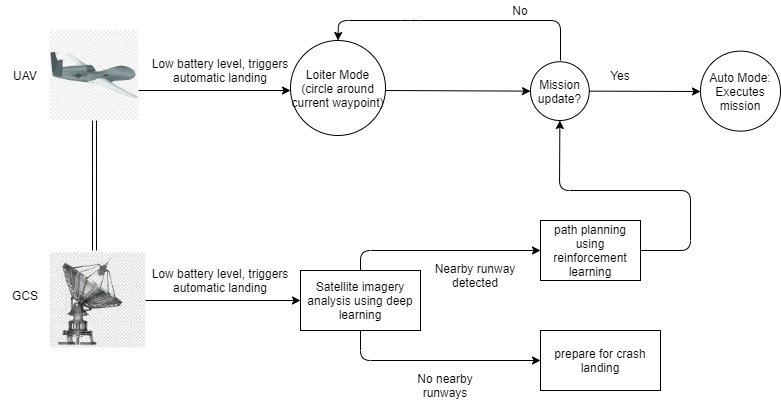
\includegraphics[width=1.0\linewidth]{flow.jpg}
\end{center}
   \caption{Illustration of the workflow of modified automatic landing}
\label{fig:long}
\label{fig:onecol}
\end{figure}
%-------------------------------------------------------------------------
%------------------------------------------------------------------------
\section{Approach}
\subsection{Datasets}
In order to properly identify a runway, we have to train a deep learning model on certain remote-sensing dataset~\cite{Author3} . There are several candidate datasets:
\begin{itemize}
\item UC Merced Land-Use
\item NWPU-RESISC45
\end{itemize}
The UC Merced Land-Use data set contains 21 classes of land-use scenes, with 100 256 x 256 images per class, and a total of 2100 images. The dataset is primarily maintained by USGS (U.S. Geological Survey) National Map of multiple states within US. This dataset offers high enough resolution of ground objects and could be used for training a baseline model.

The NWPU-RESISC45 data set contains 45 classes and has 700 images per class. In general, it is an expansion of the UC Merced Land-Use data set and features richer samples. This dataset could be used for both training, evaluation and fine-tuning. Both of the data sets meet our requirements that we need to gain better than average real time performance in recognizing any runway nearby, and NWPU-RESISC45 is actually preferred since it has more data and is likely to train a model which could potentially generalize better. In our case the smaller UC Merced Land-Use dataset was initially used due to memory bottleneck of transfer learning as well as ease of comparison for several candidate models. A smaller data set is also preferable if GPU resources are unavailable.

\subsection{Transfer Learning}
Instead of training a model from scratch, a quicker way is chosen: a network such as VGG16, VGG19, RESNET50 and Googlenet pretrained on ImageNet dataset is chosen to extract the features. The final fully-connected layers are then trained to establish a mapping between the features and the final activation output. The results are then compared and the best candidate network is chosen in the actual workflow. 

In our testing, We use Mission Planner SITL (Software In The Loop) simulation which provides a virtual plane loaded with Arduplane-4.0.0 firmware. A Dronekit python script is connected to the plane via local port 5763 and is responsible for accessing sensor data as well as giving commands. There are several reasons that Mission Planner is chosen as our GCS besides visualization purposes: one of them being the availability of the low level parameters and telemetry data. For example, we can modify the noise level and accuracy of sensors very easily in order to simulate a "real" environment. Further, the GCS itself is open-sourced and receives a lot of community support. Moreover, Mission Planner interacts with the virtual agent via Mavlink, and researchers only have to focus on high level details.

After the trained network reaches considerable testing accuracy on the training dataset, satellite images acquired by using Google Static StreetView API will be used for evaluating the performance of the network. The API allows specifying parameters (such as return image size) as well as the center geolocation coordinates. A zoom level typically between 17 to 20 is used.

\begin{figure}[t]
\begin{center}
   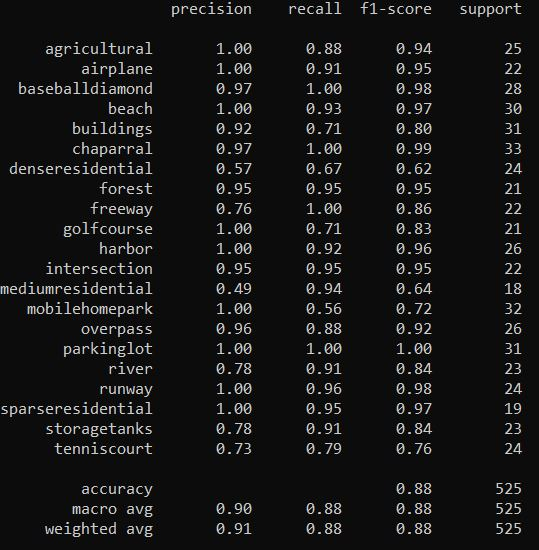
\includegraphics[width=1.0\linewidth]{vgg16.jpg}
\end{center}
   \caption{While freezing all previous layers before the final fully-connected layers, a VGG16 network trained on UC Merced  UC Merced Land-Use data set could reach 88\%-symbol; 25 training epochs are used.}
\label{fig:long}
\label{fig:onecol}
\end{figure}
\begin{figure}[t]
\begin{center}
   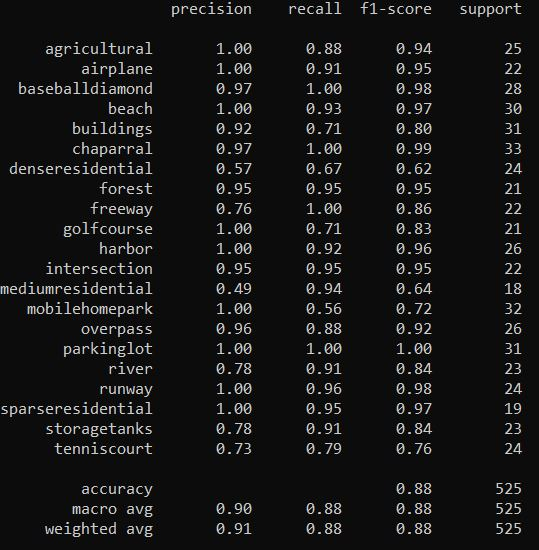
\includegraphics[width=1.0\linewidth]{vgg16.jpg}
\end{center}
   \caption{Unfreezing all previous layers, VGG16 reaches 96\%-symbol f1 accuracy; 100 training epochs are used. However, it fails to recognize a runway in suburban Australia}
\label{fig:long}
\label{fig:onecol}
\end{figure}
\begin{figure}[t]
\begin{center}
   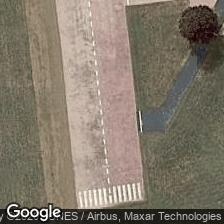
\includegraphics[width=1.0\linewidth]{sample_runway.jpg}
\end{center}
   \caption{A typical runway in suburban Australia: remote sensing image from Google Map Static API, Canberra Model Aircraft Club Flying Field}
\label{fig:long}
\label{fig:onecol}
\end{figure}
It was found that the VGG16 network using pretrained ImageNet weights could reach an f1 score of 0.88, while freezing all convolutional layers prior to the fully-connected layers. Further un-freezing of previous layers could generate an f1 score of 0.96, with satisfactory precision and recall. However, when it comes to recognizing a runway in the wild in suburban Australia, frequent mislabel occurs, leading to poor performance of the network. By analyzing the last several epochs it is obvious that the trained model is overfitting, as there were no increase in validation accuracy. A modified NWPU-RESISC45 dataset is used this time, in order to make the model generalize better. The new dataset contains only 200 images for all category except the "runway" class, thus focusing more on the recognition of that particular class.
\begin{figure}[t]
\begin{center}
   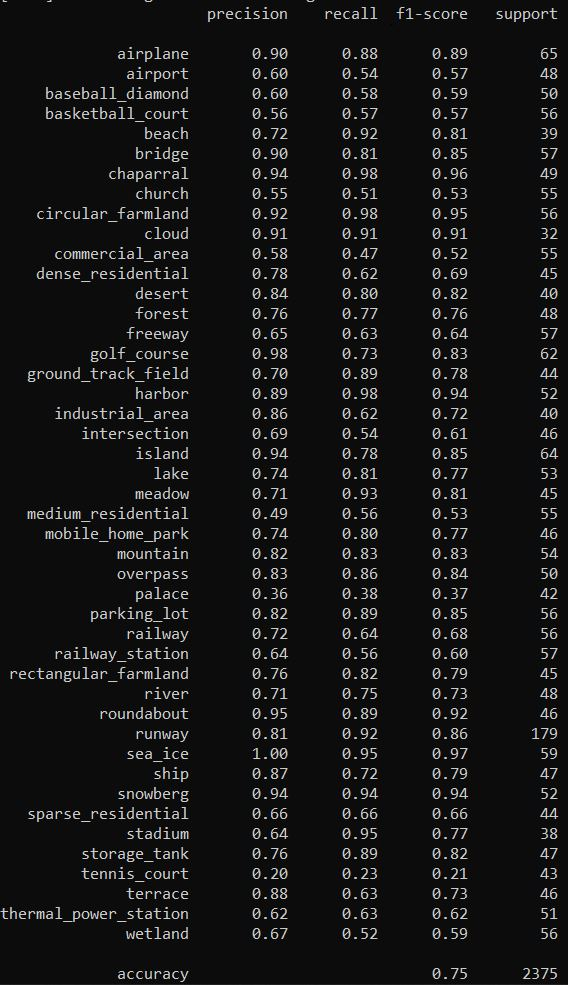
\includegraphics[width=1.0\linewidth]{modified_vgg16.jpg}
\end{center}
   \caption{fine-tuned VGG16 on modified dataset, it could be seen that the accuracy is much lower compared to the previous mode. However, the accuracy is on a larger dataset and the runway f1 score reachs 86\%-symbol, making it generalize better especially in runway recognition tasks.}
\label{fig:long}
\label{fig:onecol}
\end{figure}

In the evaluation step we have successfully detected the presence of a runway with geotextile painting. A new waypoint will be created and the UAV will navigate to that waypoint to prepare for landing.
\begin{figure}[t]
\begin{center}
   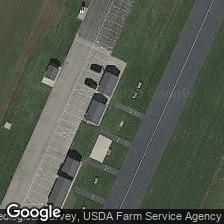
\includegraphics[width=0.5\linewidth]{runway.jpg}
\end{center}
   \caption{Successful detection of a runway in the nearby location, the latitude and longitude of that runway is also printed.}
\label{fig:long}
\label{fig:onecol}
\end{figure}
\begin{figure}[t]
\begin{center}
   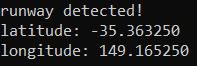
\includegraphics[width=0.5\linewidth]{detection.jpg}
\end{center}
\label{fig:long}
\label{fig:onecol}
\end{figure}
\subsection{Path Planning}
Once the runway is detected, we still need one piece of information for a successful navigation to the landing point: the orientation of the runway. Canny edge detector~\cite{Author4} is first applied to the original runway image, and then hough line transform~\cite{Author5} is applied. To get rid of the Google caption text at the bottom part of the image, the lower rows are truncated.
\begin{figure}[t]
\begin{center}
   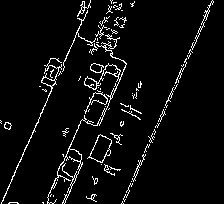
\includegraphics[width=0.5\linewidth]{edge.jpg}
\end{center}
\label{fig:long}
\label{fig:onecol}
\end{figure}
\begin{figure}[t]
\begin{center}
   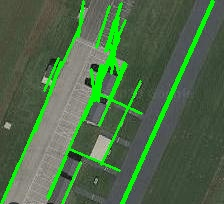
\includegraphics[width=0.5\linewidth]{hough_line_runway.jpg}
\end{center}
\caption{Lines detected by probabilistic hough line transform. The orientation of the runway is determined by counting every line's orientation angle.}
\label{fig:long}
\label{fig:onecol}
\end{figure}
Once we get the orientation of the runway, a landing waypoint could be generated by extrapolating the runway. As a result, the initial navigtion phase for the UAV is completed. The next focus is on finding an optimal path to the desired waypoint for landing. 

Unlike a chess game or a simple two-dimensional game, one obvious problem arises: the state space is too large since the aircraft is in 3D space, the aerodynamics will produce certain delay and inaccuracy while navigating to the next waypoint. Further, the potential actions are numerous. Given that most modern autopilot systems have fairly robust low level control loops, we can bypass that problem by translating it into proper ways of placing intermediate waypoints to the landing waypoint. A bounding box between the UAV's loiter position and the target waypoint is chosen, both to limit the UAV's flying area as well as providing certain degrees of freedom during its navigation. The bounding box is segmented into smaller rectangular regions, with each vertex of the rectangles a possible position for the UAV to place a waypoint. The UAV can choose actions to move up, down, left, right, upper-right, upper-left, bottom-right, and bottom-left for one grid. During each movement, a reward is given based on the vehicle's sensor data. The criterion used for determining the reward is primarily based on the remaining Euclidean distance to the target waypoint, as well as the distance traveled by the UAV. Further, for each action, the UAV will receive a slight penalty. The final reward will also be determined by the total distance traveled by the UAV, and the angle of interception to the waypoint. This is due to the fact that a fixed-wing UAV usually has a rather limited maneuverability, and bad angle of interception will cause a large deviation from the runway during landing.
\begin{figure}[t]
\begin{center}
   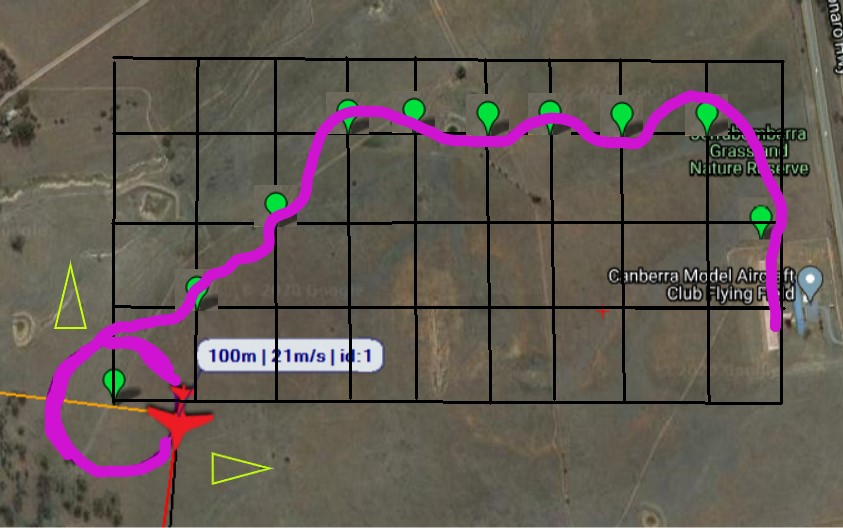
\includegraphics[width=1.0\linewidth]{path.jpg}
\end{center}
\caption{Visualization of the reduced state-space approach; a possible trajectory for navigation to the desired landing point.}
\label{fig:long}
\label{fig:onecol}
\end{figure}
A new Tensorflow Agent environment will be created from scratch by simulating the navigation process of a fixed-wing UAV loaded with Arduplane-4.0.0. The minimum turning radius of the plane is set to 5 meters, and the Dronekit script running on the background will receive the sensor data via telemetry. An agent will be trained on state of the art reinforcement learning algorithms such as DQN~\cite{Author6}, DDQN~\cite{Author7}, DDPG~\cite{Author8} and PPO~\cite{Author9}, using tf-agents API.

\subsection{Criteria}
A proper reward calculation is necessary for the UAV to follow the desired trajectory. In the previous works, SPL~\cite{Author10}(Success Weighted by (normalized inverse) Path Length) is choesen as the evaluation technique for giving out rewards:
\begin{equation}
\frac{1}{N} \sum_{i=1}^{N} S_i \frac{l_i}{max(p_i, l_i)}
\end{equation}
in which $S_i$ is a boolean value indicative of whether or not the episode is successful or not, $l_i$ denotes the shortest path distance from the agent's starting position to target position in the corresponding episode, and $p_i$ is the actual length taken by the agent in that episode. A similar approach could be adopted. Since our agent (UAV) can travel freely in 3D space, we can regard the shortest path distance from its starting to ending (landing) waypoint as the 2D Euclidean distance between those two waypoints. Besides, we want to penalize the UAV if its interception angle deviates too large from the runway entry point. Our modified SPL, a.k.a. Land-SPL is thus:
\begin{equation}
\frac{1}{N} \sum_{i=1}^{N} S_i \frac{l_i}{max(p_i, l_i)} - e^{k(\theta - \phi)}
\end{equation}
in which $S_i$ denotes whether the UAV has successfully navigated to the vicinity of the landing waypoint (within a radius of 10 meters), $p_i$ denotes the actual distance travelled by the UAV (proportional to the fuel/battery power consumed), $l_i$ is the Euclidean distance between the initial loiter waypoint to the landing waypoint in a 2D plane, and $\theta - \phi$ is the deviation angle from the waypoint orientation. Notice here $k$ is a scalable hyperparemeter and could be adjusted in actual training.

Once the UAV has reached the vicinity of the entry point, the last waypoint it has placed will be overwritten by the landing waypoint. Considering that a common UAV will take less than 2 seconds in traveling 10 meters, the difference in fuel consumed will be negligible. 
\section{Experiments and Results}
pretrained VGG16, Resnet50, and Alexnet as well as self-trained Googlenet is tested on the runway dataset. Googlenet, which has Inception modules incorporated, is far from ideal, and the testing accuracy is around 33-34 \%. That could be partially attributed to the large compression on the 256 by 256 remote sensing images that largely degrades high level details of of the image. A runway is hardly distinguishable from an ordinary road except in the patterns near the end points. Thus, networks with large input size is more preferrable as they could preserve the features necessary for successful classification. In general, Resnet-50 is a compromise for both performance and speed of classification, while Alexnet, on the other hand, offers the highest f1 score but the speed is way too slow (approx. 5-6 sec per image), making it less desirable for real-time classification tasks.



In the simulation, the UAV is able to follow a nearly-optimal path and perform a successful landing. However, for now the path planning algorithm is rather hard coded and the agent has not been trained extensively to be able to figure out the optimal path. 

\begin{table}
\begin{center}
\begin{tabular}{|l|c|}
\hline
Method & f1 score\\
\hline\hline
VGG16 & 86\% \\
Resnet & 94\% \\
Alexnet & 97\%\\
Googlenet & 33.5 \%\\
\hline
\end{tabular}
\end{center}
\caption{Results.   performance of different networks on modified NWPU-RESISC45 data set.}
\end{table}

%-------------------------------------------------------------------------
\section{Future works}
The new automatic landing feature is aimed at replacing Ardupilot's current automatic landing feature, and will be one of the \href{https://ardupilot.org/dev/docs/roadmap.html}{Ardupilot Roadmap for 2020/2021}. Algorithm robustness both in runway detection and the path planning needs to be enhanced. The runway detection is mostly successful in asphalt as well as geotextile painted scenarios, but not so ideal if the runway has not been painted for a long time. A larger dataset with handcrafted features will be used for training to cover those scenarios. Further, a robust 2D path planning agent will be used in the training process and further implementations will consider 3D path planning, taking altitude into consideration.

An improvement to the general workflow might also be taken into consideration: a modified YOLOv4~\cite{Author11} will be used to replace the aforementioned "outdated" networks, to both recognize the runway and extract its location in the picture. Compared to previous YOLO versions, YOLOv4 offers much higher speed which could be used to scan a large area of satellite imagery. The increased accuracy in runway localization could also improve the generation of landing waypoint. Additional features include the scenario in which multiple runways are detected, the closest runway will be chosen to save fuels for the UAV, as well as shutting down unnecessary sensors to save power.

The new landing feature will also be tested on actual robots and UAVs, and their corresponding performance will be recorded and used for further improvements and bug fixing.
%-------------------------------------------------------------------------
\section{Acknowledgements}
The author wishes to thank Ardupilot project team, as well as Mission Planner project which offers a suitable environment for robotics simulation.

\begin{table*}
\begin{center}
\begin{tabular}{|l|c|c|}
\hline
Student Name & Contributed Aspects & Details \\
\hline\hline
Team Member 1 & Data Collection Implementation & Trained the CNN network for runway recognition and coded the Dronekit script \\
\hline
\end{tabular}
\end{center}
\caption{Contributions of team members.}
\label{tab:contributions}
\end{table*}

{\small
\bibliographystyle{ieee_fullname}
\bibliography{egbib}
}


\end{document}
